\documentclass[11pt, a4paper]{article}
%\usepackage{proj1}
\usepackage{natbib}
\usepackage{fancyhdr}  
\usepackage{subcaption}
\usepackage{caption}
\usepackage{graphicx}
\usepackage{numprint}
\usepackage{multirow}
\linespread{1.25} 
\setlength{\parindent}{0cm}
\graphicspath{{Images/}}
\usepackage{hyperref}
\usepackage{amsmath}
\usepackage{amsfonts}
\usepackage{amssymb}
\usepackage{amsthm}
\usepackage{mathtools}
\usepackage{commath}
\usepackage{bbm}

%\usepackage[sc,osf]{mathpazo}
\usepackage{subcaption}
\usepackage[a4paper, top=1in, left=1.0in, right=1.0in, bottom=1in, includehead, includefoot]{geometry} %Usually have top as 1in

\usepackage{listings}
\usepackage{color} %red, green, blue, yellow, cyan, magenta, black, white
\definecolor{mygreen}{RGB}{28,172,0} % color values Red, Green, Blue
\definecolor{mylilas}{RGB}{170,55,241}


\hypersetup{colorlinks,linkcolor={black},citecolor={blue},urlcolor={black}}
\usepackage{color}
\urlstyle{same}


\theoremstyle{definition}
\newtheorem{definition}{Definition}[section]

\newcommand{\adja}{q_a}
\newcommand{\adjb}{q_b}
\newcommand{\adjaB}{q_{a,\partial \Omega}}
\newcommand{\adjbB}{q_{b,\partial \Omega}}
\newcommand{\adjB}{q_{\partial \Omega}}
\newcommand{\Adja}{\mathbf{p}}
\newcommand{\Adjb}{q}
\newcommand{\adj}{q}
\newcommand{\Adjc}{{q}_{\partial \Omega}}
\newcommand{\ra}{\rho_a}
\newcommand{\rb}{\rho_b}
\newcommand{\w}{\mathbf{w}}
\newcommand{\f}{\mathbf{f}}
\newcommand{\ve}{\mathbf{v}}
\newcommand{\n}{\mathbf{n}}
\newcommand{\h}{\mathbf{h}}
\newcommand{\K}{\mathbf{K}}
\newcommand{\hr}{\widehat \rho}

\begin{document}
	\section{Sedimentation Optimization}
	We have $N = 40$ and $n = 30$ for each shape. We choose the ODE tolerance to be $10^{-7}$ and the optimization tolerance is $10^{-3}$.
	I fixed the problems with the implementation of the sedimentation optimization code. First, I tested whether setting $\hr = \rho_{FW}$ would converge within one iteration. This happened. 
	Then I set up a test problem which sets $\hr$ to be the forward solution for $V_{ext} = ay$, where $a = 0.1$, as in Archer's paper. Then I set up the optimization forward problem to be such that $a = 0.01$ and $\w = \mathbf 0$. We expect the control to act downward, since the strength of gravity $a$ is decreased.
	We also expect that the cost $\mathcal J$ is decreasing from the baseline $J_{FW}$ when optimizing.
	For $\beta = 10^{-3}$ and $\beta = 10^{-1}$ this works well.
	When $\beta = 10^{-3}$ we get $J_{FW} = 0.4955$ and $J_{Opt} = 0.0556 $. 
	The results can be seen in Figures \ref{F1}, \ref{F2} and \ref{F3}.
	\begin{figure}[h]
		\centering
		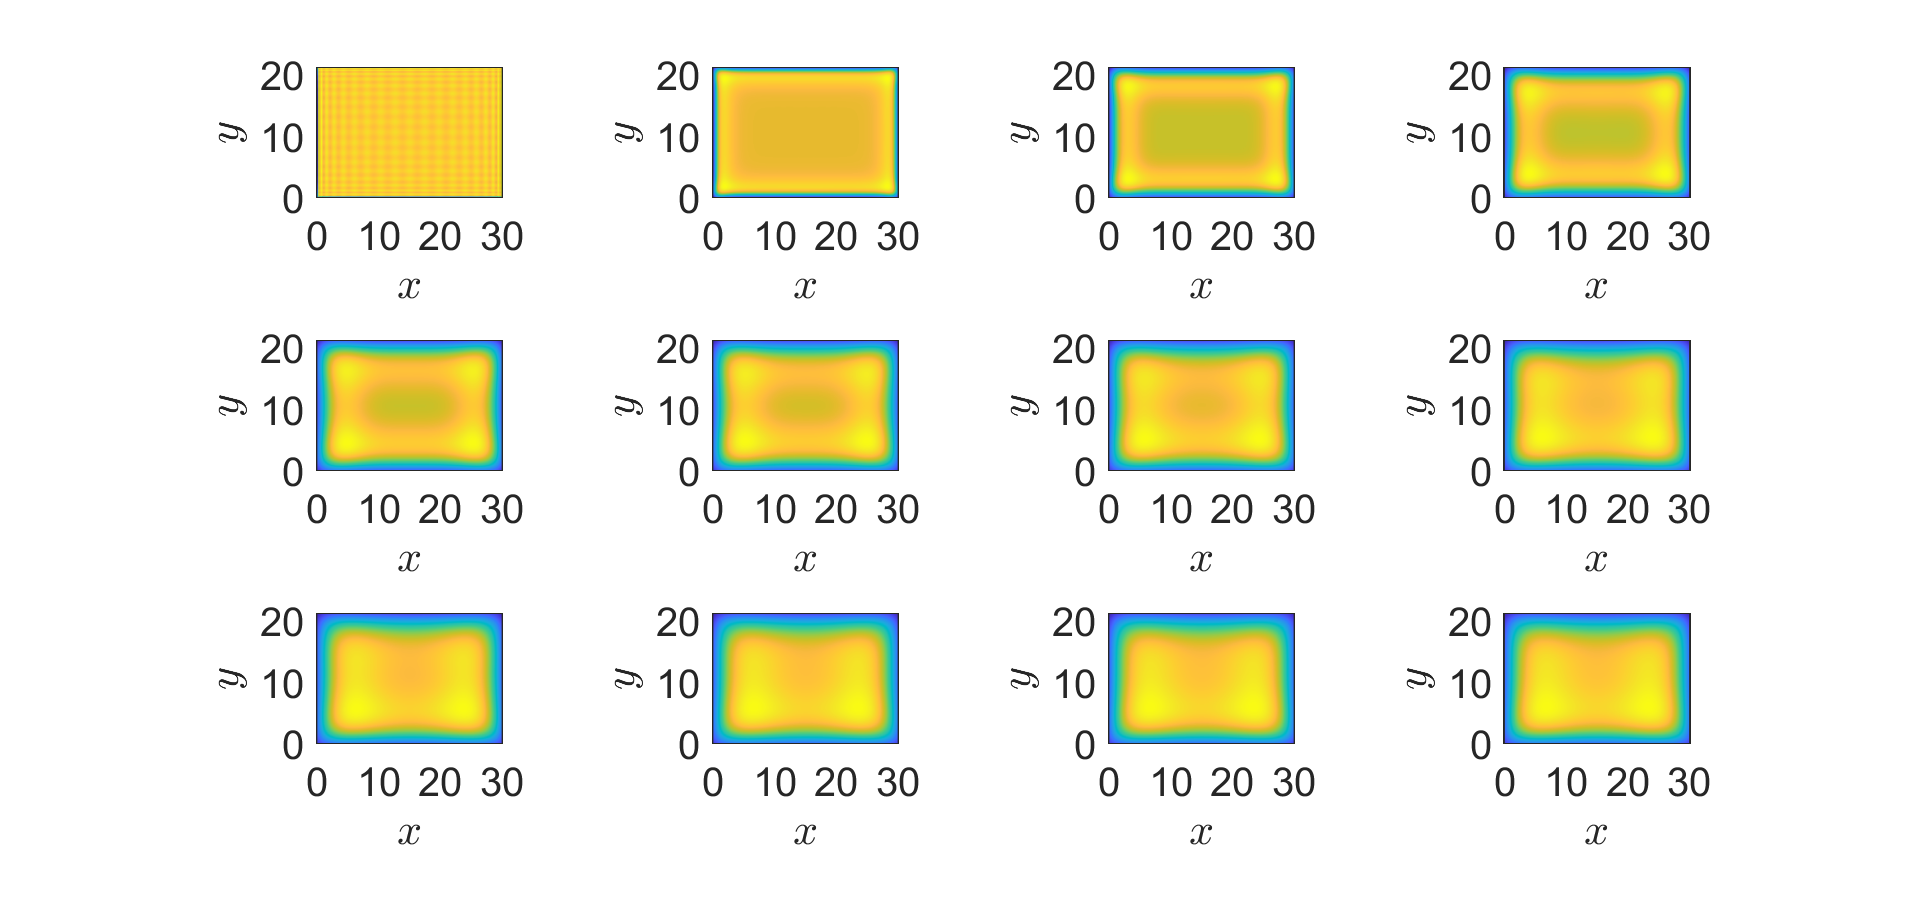
\includegraphics[scale=0.35]{F1.png}
		\caption{Forward $\rho$ for $a = 0.01$} 
		\label{F1}
	\end{figure}	
	\begin{figure}[h]
		\centering
		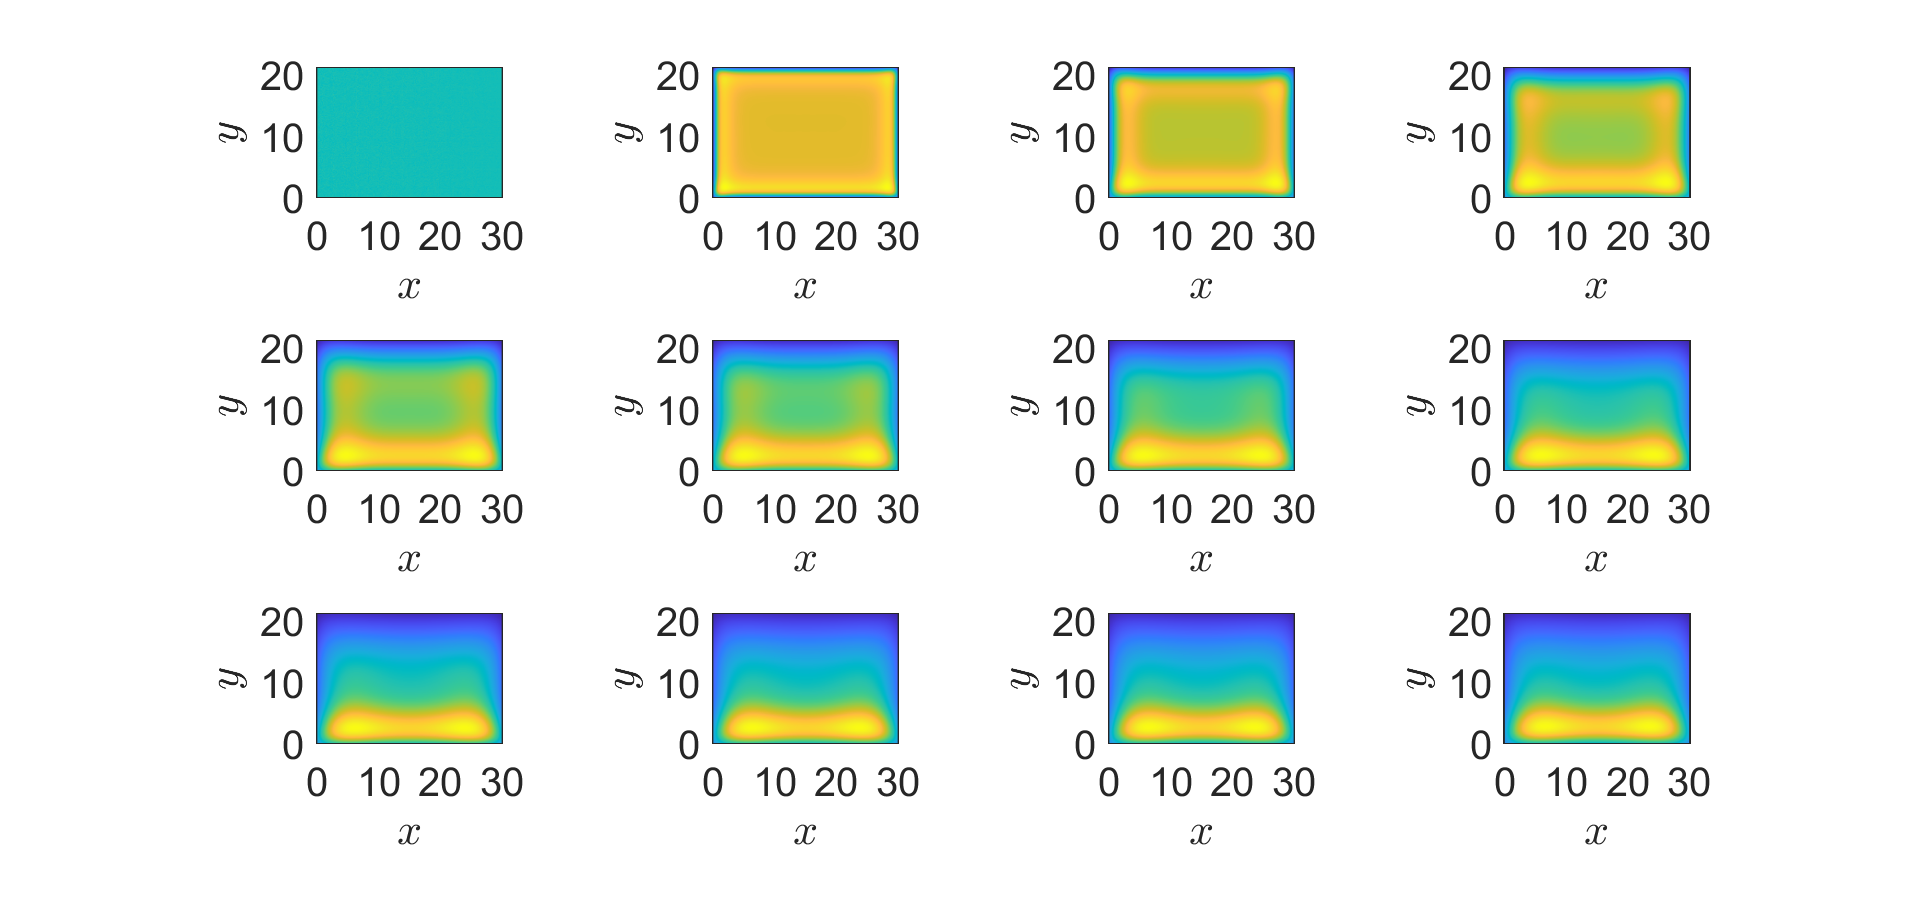
\includegraphics[scale=0.35]{F2.png}
		\caption{Optimal $\rho$ for $a = 0.01$} 
		\label{F2}
	\end{figure}
	\begin{figure}[h]
		\centering
		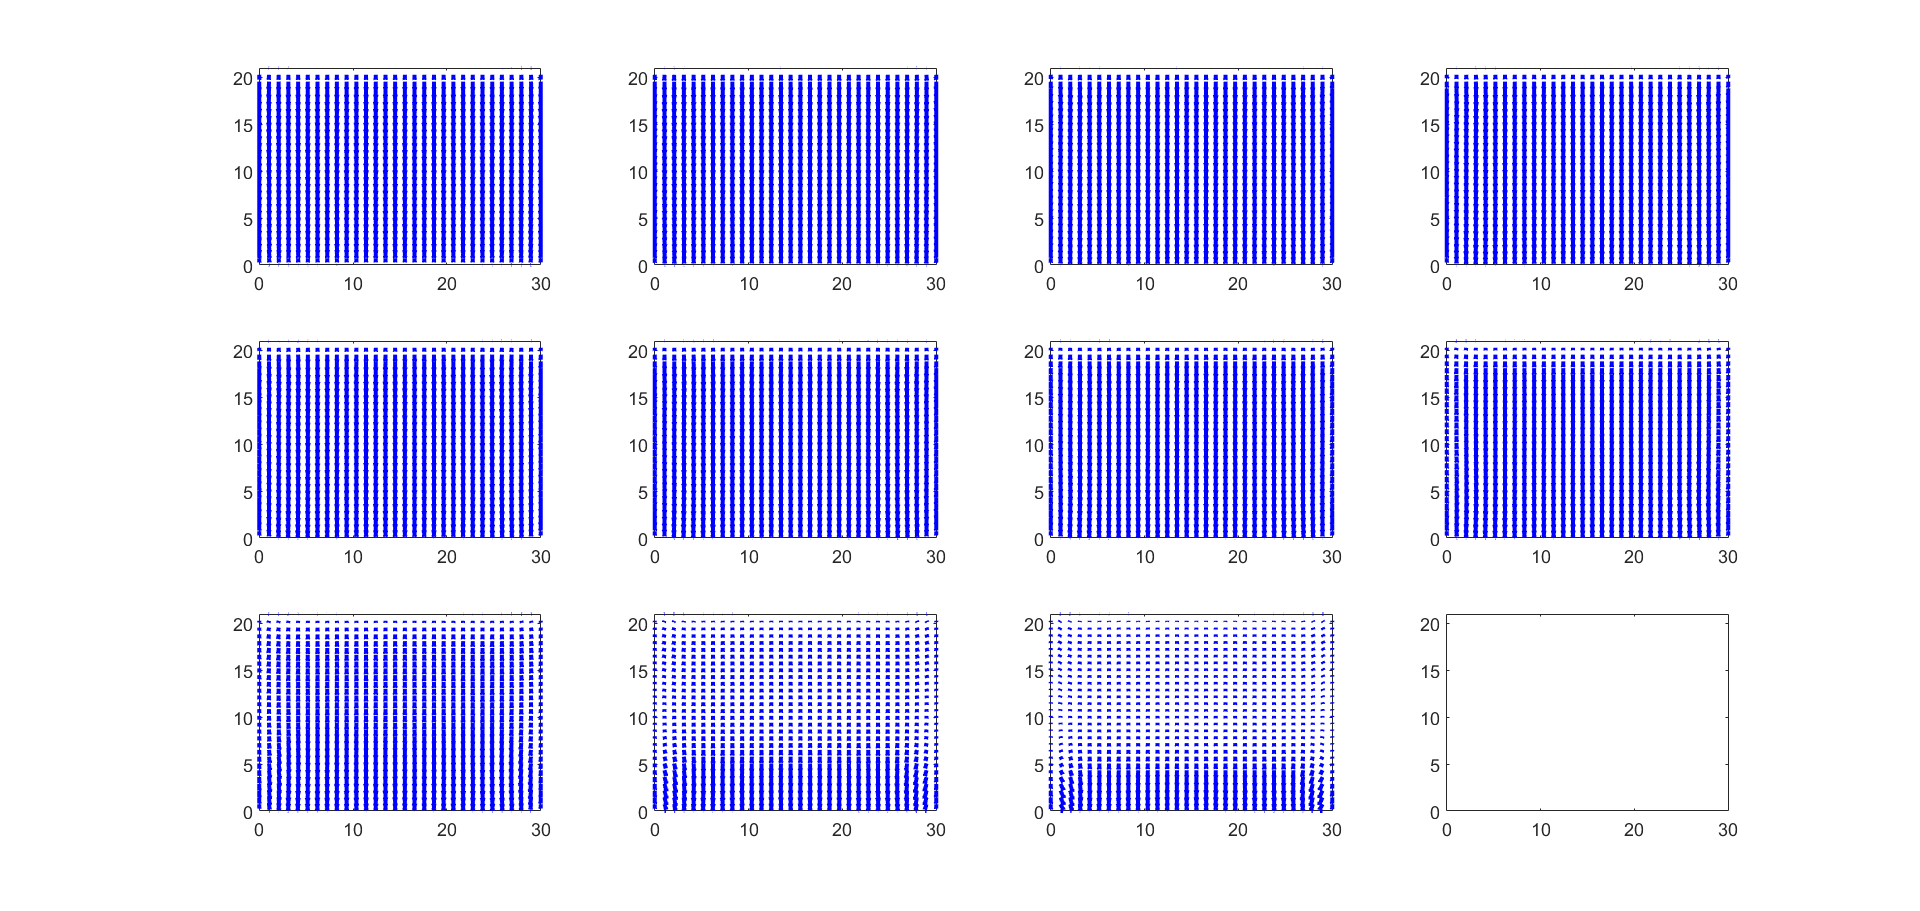
\includegraphics[scale=0.35]{F3.png}
		\caption{Optimal Control for $a = 0.01$} 
		\label{F3}
	\end{figure}
	
	
	
	\subsection{Multishape}
	Just to test whether the multishape OCP works now (since there have been issues in the past which have been fixed when fixing another bug). We have $N =20$ and $n = 30$ for each shape. We choose the ODE tolerance to be $10^{-7}$ and the optimization tolerance is $10^{-3}$.
	We choose the target with $a=0.1$ and the forward problem with $0.099$, so that we get quick convergence, since we just want to see whether the method is working.
	We get $J_{FW} = 4.4833 \times 10^{-5}$ and $J_{Opt} = 2.6884 \times 10^{-6}$. The results can be seen in Figures \ref{F4} and \ref{F5}.
	\begin{figure}[h]
		\centering
		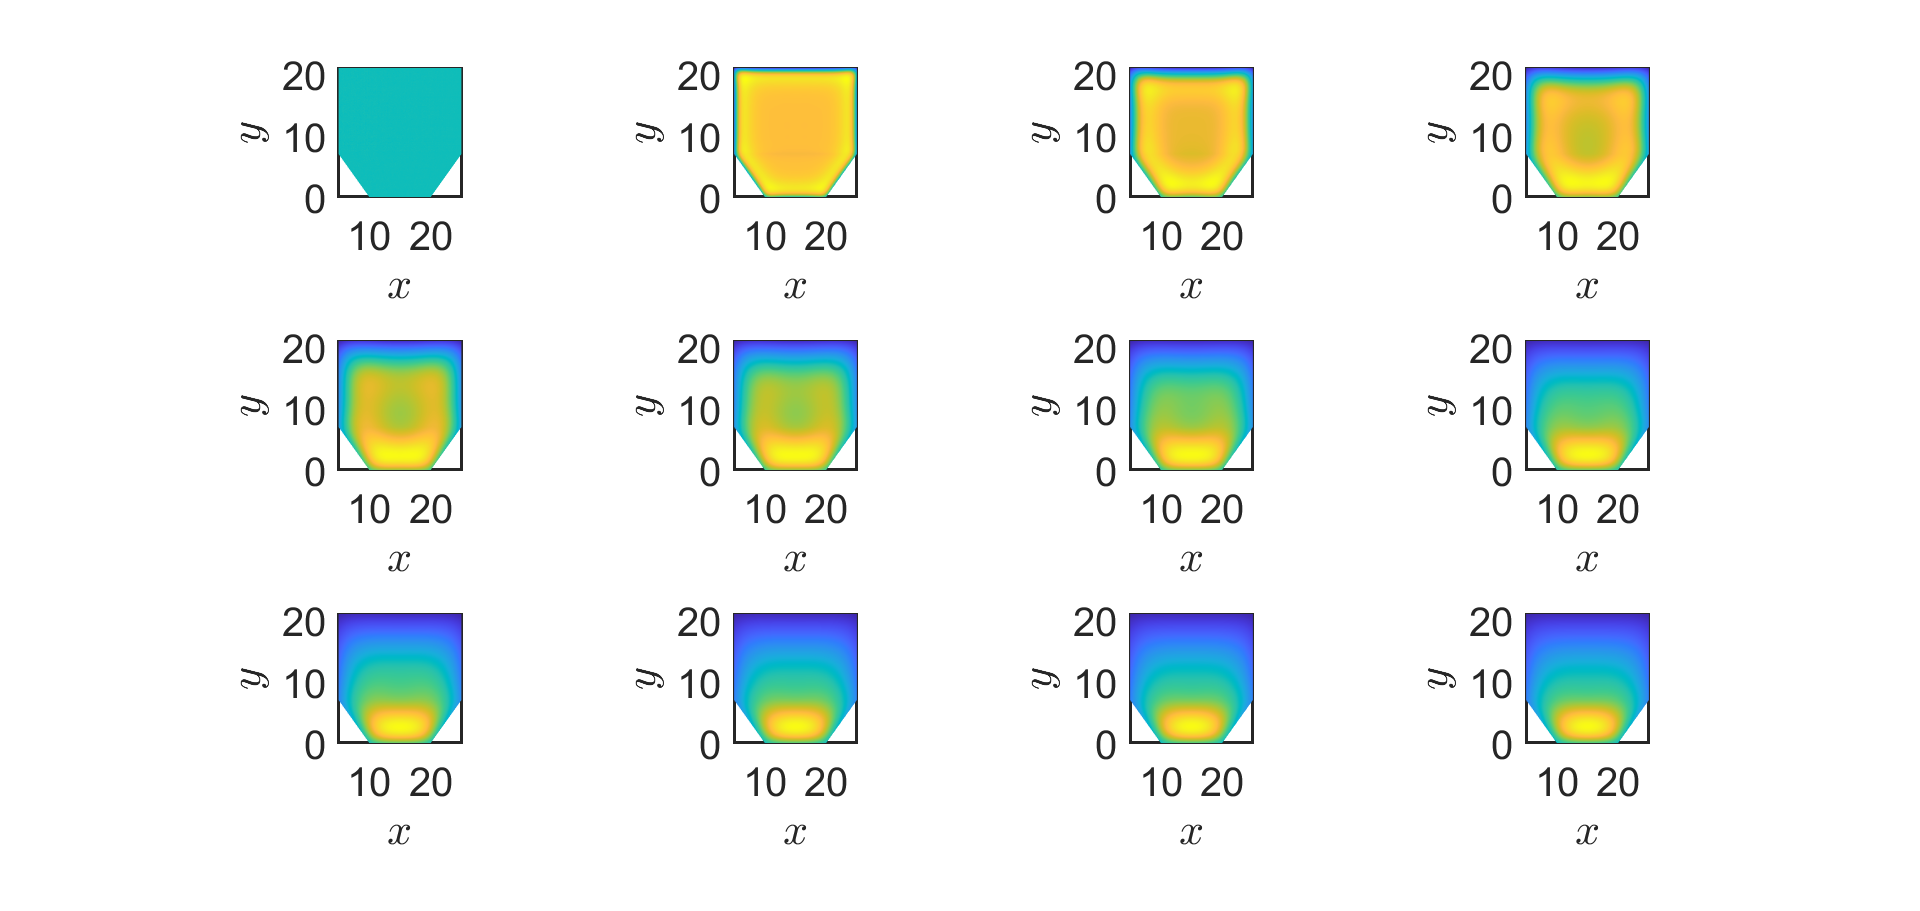
\includegraphics[scale=0.35]{M1.png}
		\caption{Optimal $\rho$ for $a = 0.099$} 
		\label{F4}
	\end{figure}
	\begin{figure}[h]
		\centering
		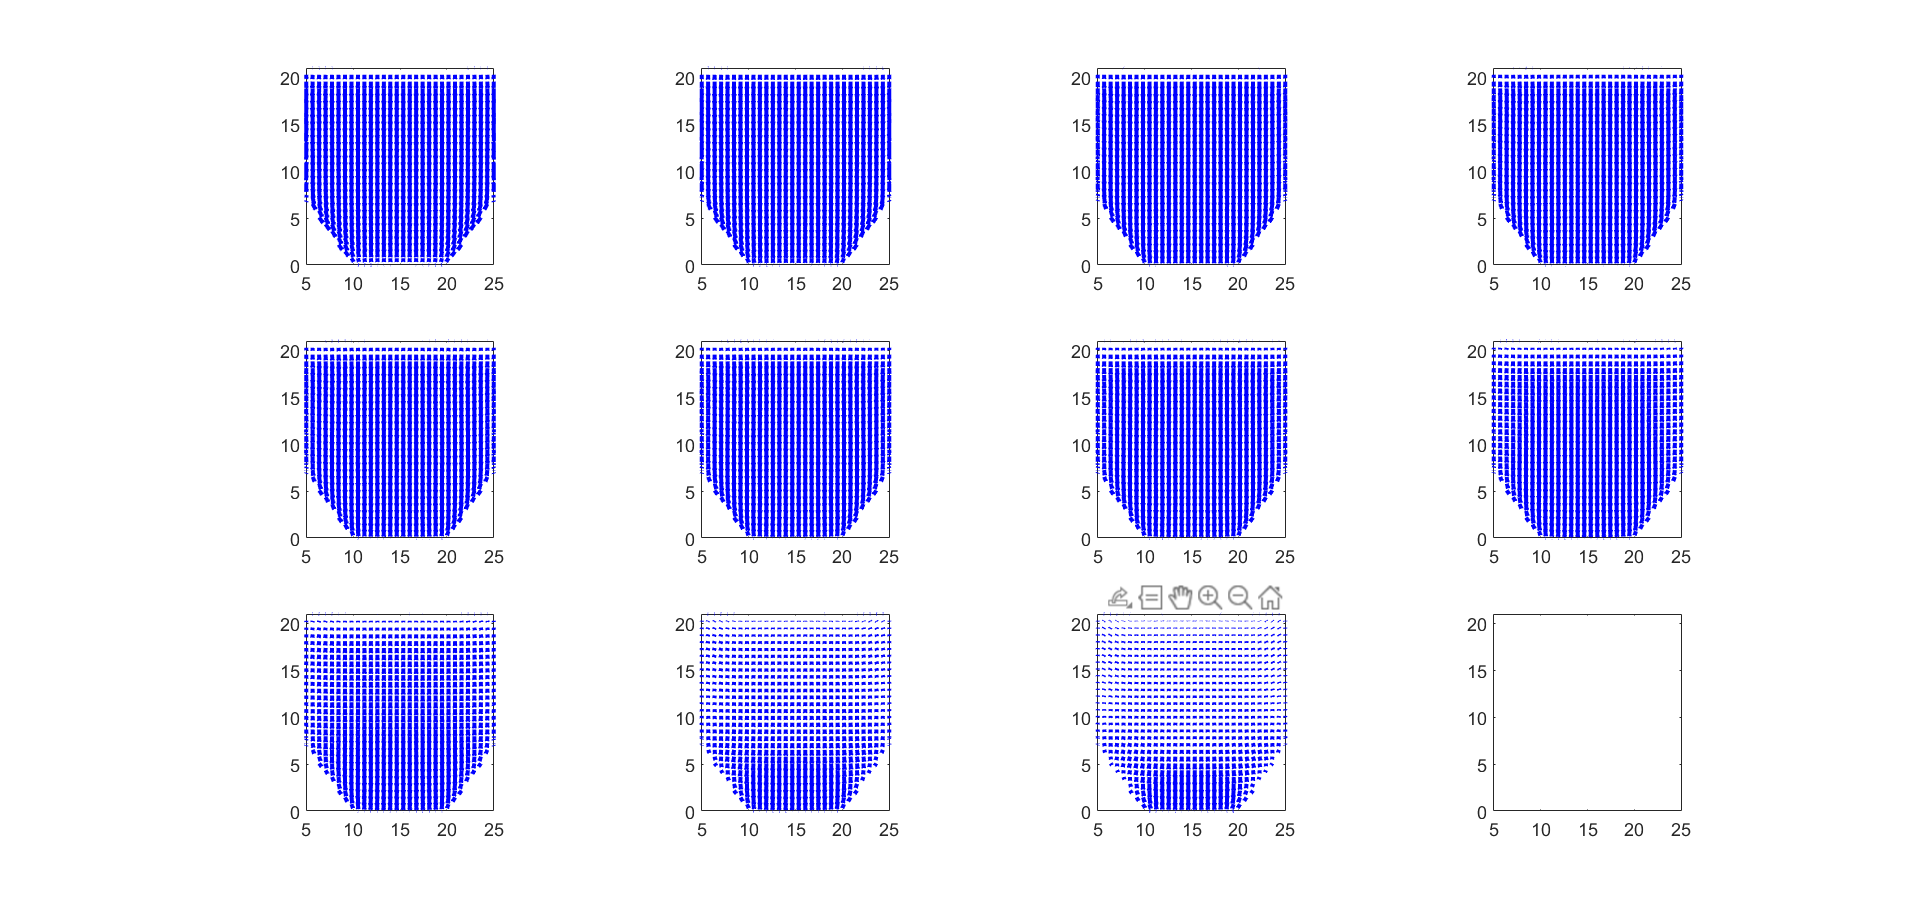
\includegraphics[scale=0.35]{M2.png}
		\caption{Optimal Control for $a = 0.099$} 
		\label{F5}
	\end{figure}
	
	
	\section{Time-independent control}
	We now use the example with the same configurations as in the first section. The difference will be that the gradient equation is:
	\begin{align*}
		\w = - \frac{1}{\beta}\int_0^T \rho \nabla q dt.
	\end{align*}
	This means, we get a $\w$ which is averaged over the time horizon and therefore time independent. This seems to work well. $J_{FW} = 0.4855$ and $J_{Opt} = 0.0733$. The results can be seen in Figures \ref{F6}, \ref{F7} and \ref{F8}.
	
		\begin{figure}[h]
		\centering
		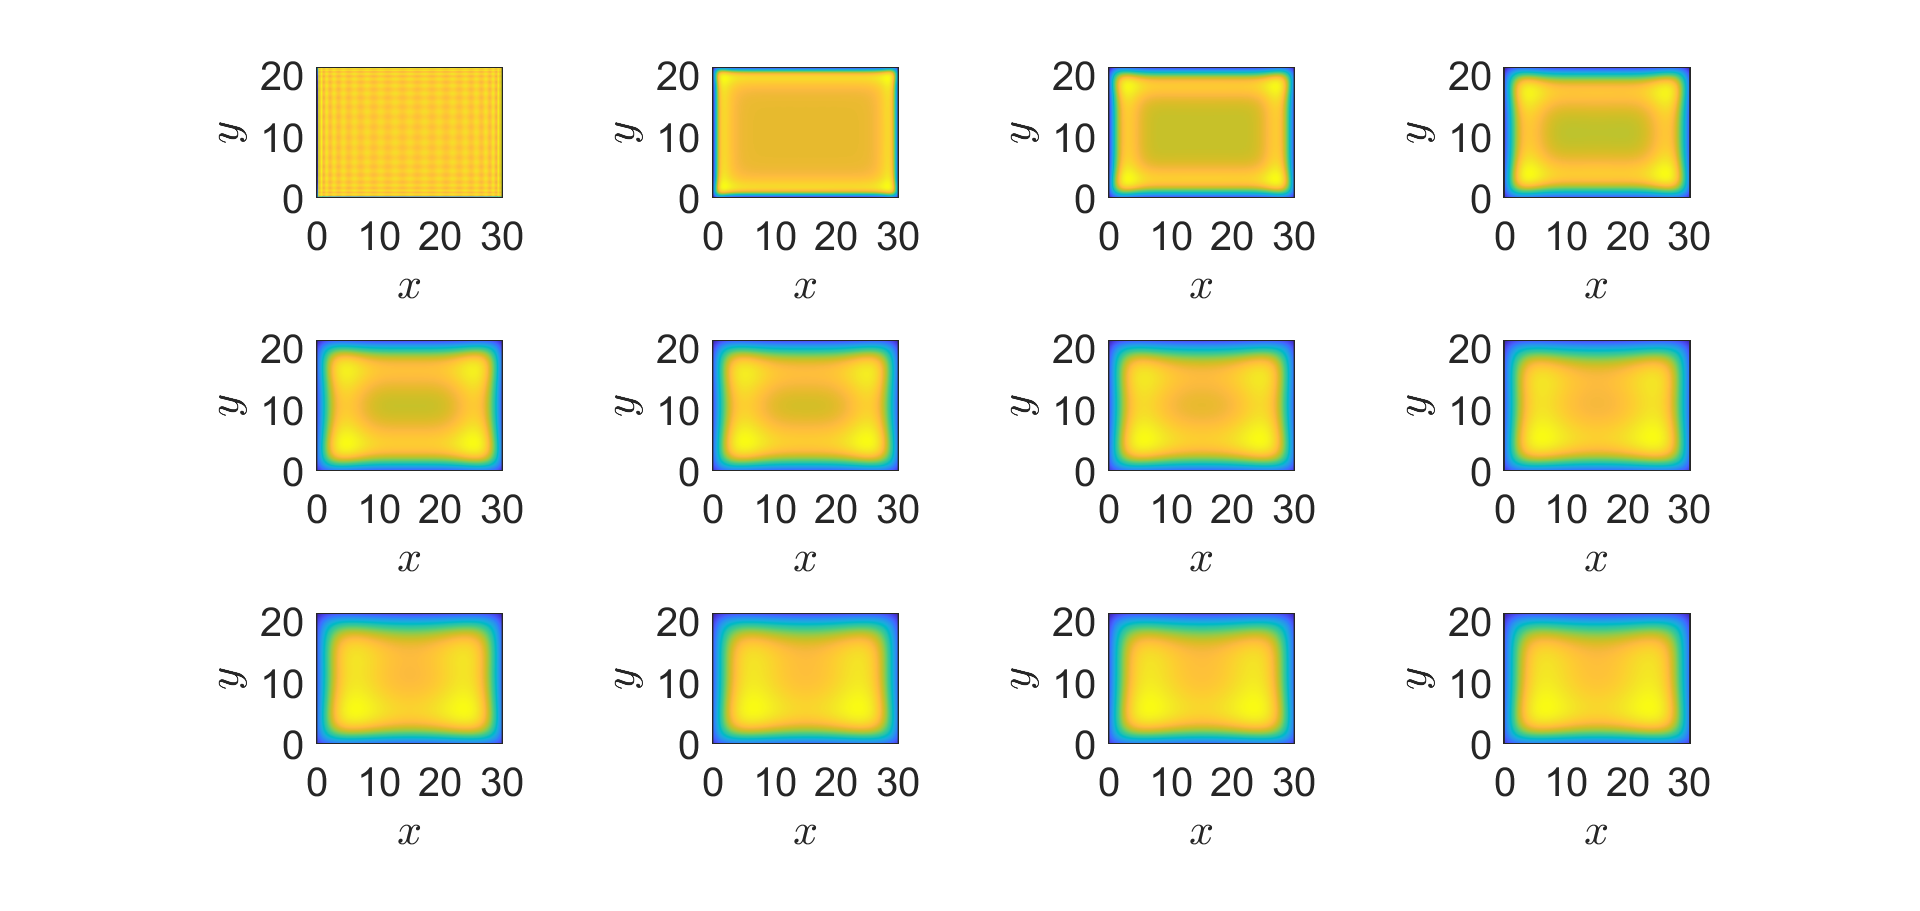
\includegraphics[scale=0.35]{C1.png}
		\caption{Time-independent; Forward $\rho$ for $a = 0.01$} 
		\label{F6}
	\end{figure}	
	\begin{figure}[h]
		\centering
		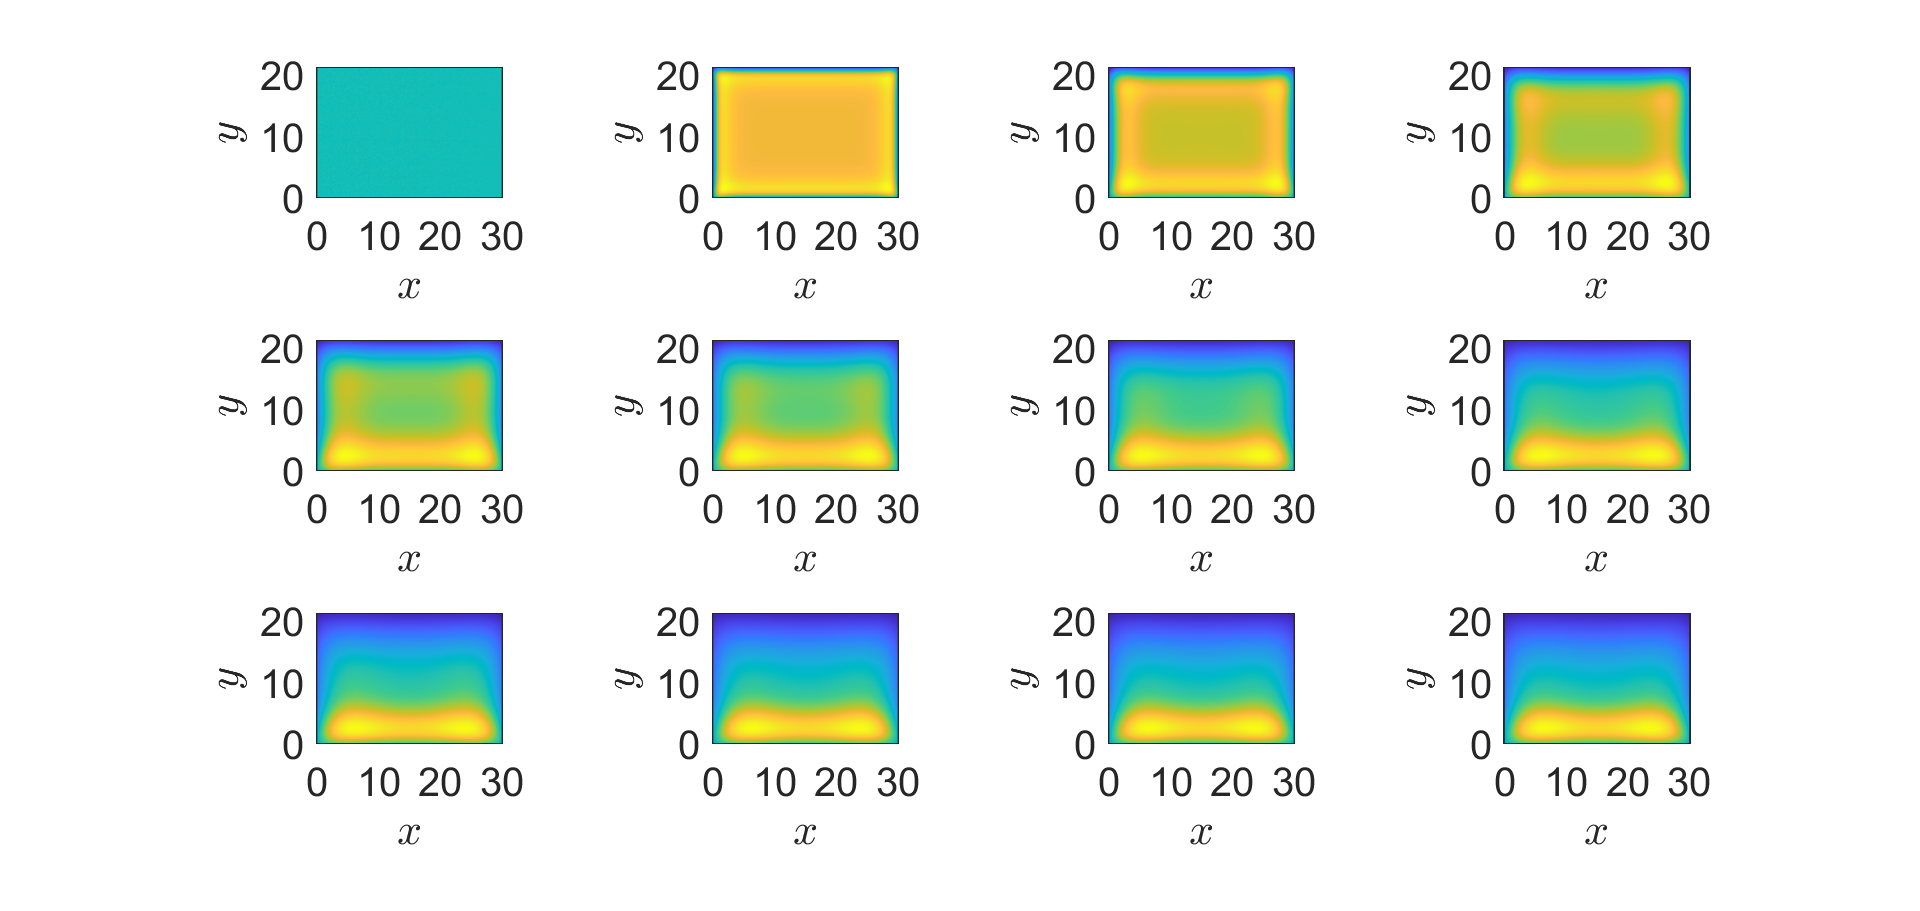
\includegraphics[scale=0.35]{C2.png}
		\caption{Time-independent; Optimal $\rho$ for $a = 0.01$} 
		\label{F7}
	\end{figure}
	\begin{figure}[h]
		\centering
		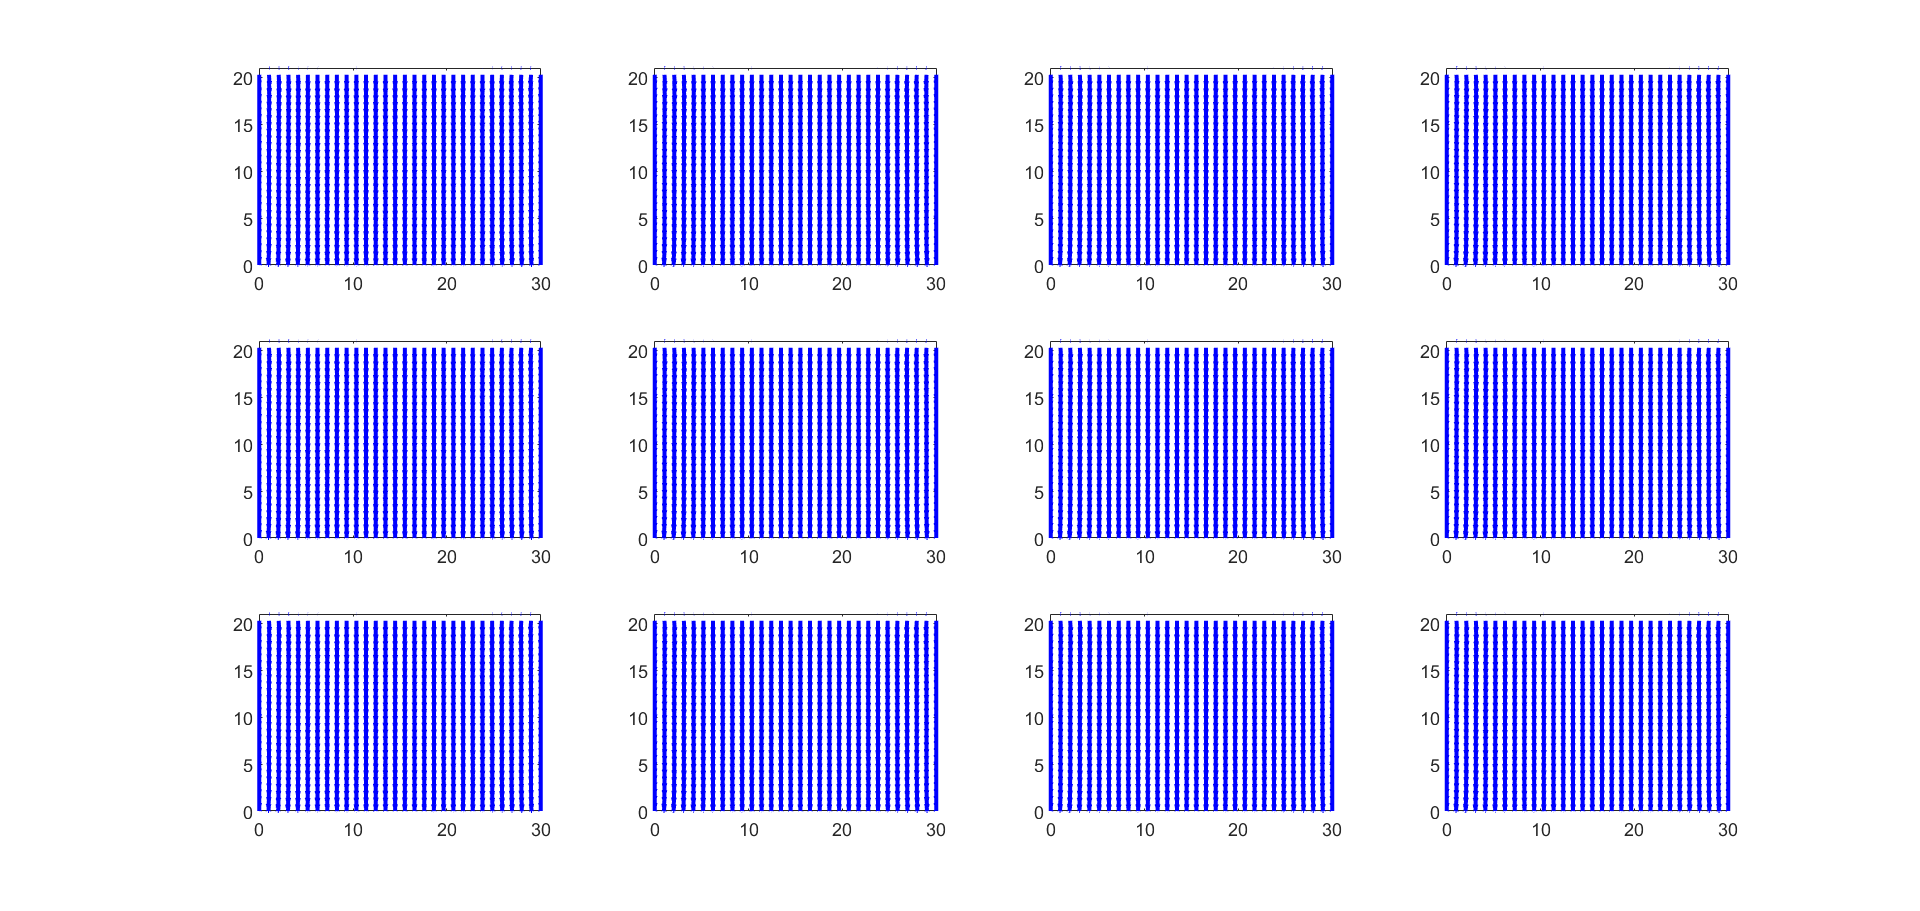
\includegraphics[scale=0.35]{C3.png}
		\caption{Time-independent; Optimal Control for $a = 0.01$} 
		\label{F8}
	\end{figure}
	
	
	
	
	
\end{document}